%\documentclass[a4paper]{article}
\documentclass[journal]{IEEEtran}

\usepackage[pdftex,pdfauthor={Shabaz Sultan, Chi Chun Wan, Boudewijn Zwaal},pdftitle={Airline sc},colorlinks=true, linkcolor=black,          % color of internal links
    citecolor=black,        % color of links to bibliography
    filecolor=black,      % color of file links
    urlcolor=black   ]{hyperref}
\usepackage[pdftex]{graphicx}
\usepackage{amsmath}
\usepackage{float}

\author{Chi Chun Wan -- 2525244\\
Shabaz Sultan -- 2566703\\
Boudewijn Zwaal -- 1897527}
\title{Airline Scheduling with Simulated Annealing}
\begin{document}
\maketitle



\begin{abstract}
%\boldmath
Abstract text to go here.
\end{abstract}


\section{Introduction}
In this report, we will produce a flight schedule for six airplanes for the airline Mokum Airways with as goal to maximize the passengers-kilometers. In order to obtain the best flight schedule, we use heuristics algorithms to analyze all the possible tours and find the optimal one.\\
Mokum Airways, a newly created Dutch airline based in Amsterdam, has landing rights for 28 destinations around Europe. \\
\begin{figure}[!h]
\centering
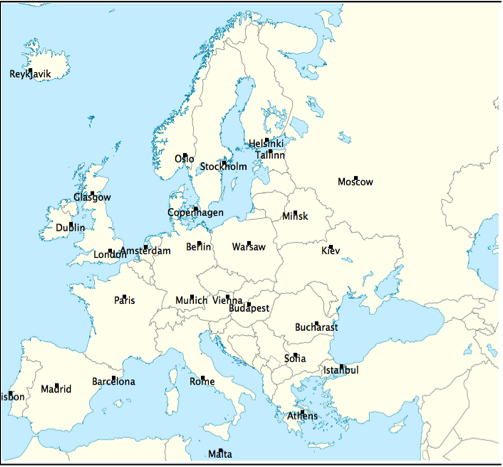
\includegraphics[width=2.5in]{europe}
\caption{Mokum Airways destinations}
\label{fig:europe}
\end{figure}
The problem is how their flight schedule should look like with as goal to maximizes the number of passenger-kilometers. The number of passenger-kilometers is the number of passenger times the number of kilometers in the air. This goal is important for the airline, because the number of passenger-kilometers determines the profit. \\
The airline has a fleet of six Airbus A321 aircrafts with speed of 800km/h, capacity of 199 and range of 3199 km.  The take-off and landing take place between 02:00 and 06:00 and docking time and refuel time will take one hour. Moreover, once per day the plane needs to land in the home-base for the crew-change. The flight schedule has to be a cycle, so the start point and the end point of the route has to be the same. \\

\section{Background}
Some example citations \cite{Langerman1997} \cite{Lohatepanont2004} \cite{Mashford2001}.
\section{Algorithm}
To deal with the problem, we use two heuristic algorithms, namely hill-climbing and simulated annealing for six airplanes and one algorithm brute force for one airplane.

\subsection{Brute-force}
Brute-force is a problem-solving technique that consists of systematically enumerating all possible candidates for the solution and checking whether each candidate satisfies the problem's statement. In our case, we check all the possible tours by using a tree structure, where the node represents the destinations. A representation of the tree is given in figure~\ref{fig:tree}.\\
\begin{figure}[!h]
\centering
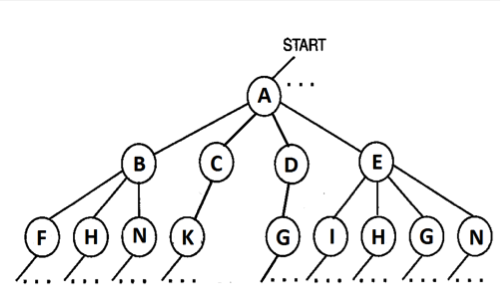
\includegraphics[width=2.5in]{tree}
\caption{Tree data structure}
\label{fig:tree}
\end{figure}
\\
An advantage of this algorithm is that the solution found, also is  the optimal solution. A disadvantage is that the run time will increases a lot to find a solution, when the state space is big. Therefore, we add branch and bound to the algorithm. The branch and bound algorithm has a upper-and lower bound. The upper bound is the theoretical maximum passengers-kilometer score and the lower bound is the best founded score so far for every step. For every position in the tree, we calculate what the maximum score is that can still be obtained from that position. If the score is lower than the current lower bound. We will not look further anymore from that position. This has as result that it will make the possibilities smaller and therefore a lower run time. 
\subsection{Hill-climbing}
Hill-climbing is an iterative algorithm that starts with an arbitrary solution to a problem, then attempts to find a better solution by changing a single element of the solution. If the change produces a better solution, an incremental change is made to the new solution, repeating until no further improvements can be found.\\
In the case of our problem, a flowchart is made in figure~\ref{fig:flowchart_hc}.\\
\begin{figure}[!h]
\centering
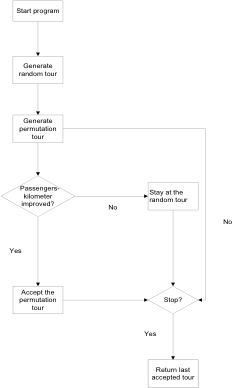
\includegraphics[width=2.5in]{flowchart_hc}
\caption{Flowchart Hill-climbing}
\label{fig:flowchart_hc}
\end{figure}
\\
We start with an initial random tour. To find a better solution, we permutate the tour by randomly selecting a sub-tour in the initial tour and replace it with another possible valid sub-tour. Care is taken to not remove the home-base airport from the tour. The score of the passenger-kilometers for the initial tour is stored in a variable best score. If the score of the permutation tour is higher than the score of the arbitrary tour, the score of the permutated tour will be the new best score and the permutation tour will be accepted, otherwise the best score will stay the same and we will stay at the previous tour. This process is repeated until no further improvements can be found and the best tour is the last accepted tour. When applied to multiple planes, first one of the planes in the system is randomly chosen and its flightplan (tour) is permutated. The total score of all airplane tours is then calculated and compared to the previous best score. If it improves on said score, the new tour is accepted.\\
A disadvantage of hill-climbing is that it is good for finding a local optimum, but it is not guaranteed to find the best possible solution (global optimum). To avoid this disadvantage, we use a different algorithm, simulated annealing. \\
\subsection{Simulated Annealing}
In case of simulated annealing, it’s almost the same as hill climbing except when the solution is not improved, this solution will be accepted with a probability P. The probability is based on the number of iterations and the temperature. As the number of iterations increases, the temperature goes down and the probability will decrease. \\
In figure~\ref{fig:flowchart_sa}, the flowchart of hill-climbing is adjusted in simulated annealing.\\
\begin{figure}[!h]
\centering
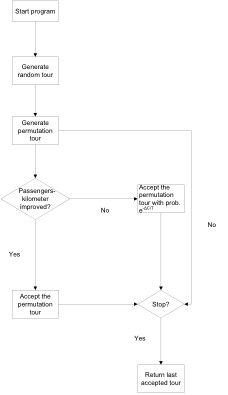
\includegraphics{flowchart_sa}
\caption{Flowchart Simulated Annealing}
\label{fig:flowchart_sa}
\end{figure}
\\
In the case when the passengers-kilometer score is not improved, you will accept the permutation tour with probability $P = e^{\frac{−\Delta C}{T}} $, where ∆C = score of the permutation tour − score of the current best tour and $T = 0, 999^i * T_0$ with $i$ is the number of iterations and $T_0$ is the start temperature 50.000.
 This probability will decrease with the number of iterations. Thus when the number of iterations increases, the temperature goes down. When temperature is high, the system will choose new states more or less at random, but as the temperature lowers this algorithm will go to hill-climbing. 
\section{Result}
\section{Analysis}
To analyze the quality of the heuristic algorithms, Hill-climbing and simulated annealing. We use the result of the brute force for one airplane as reference, since the result is the global maximum. In graph 1, the RMSE of the score for simulated annealing is plotted. When the iterations increase, the RMSE will decrease. The number of iterations depends on the cooling rate, a lower cooling rate will 
\begin{figure}[!h]
\centering
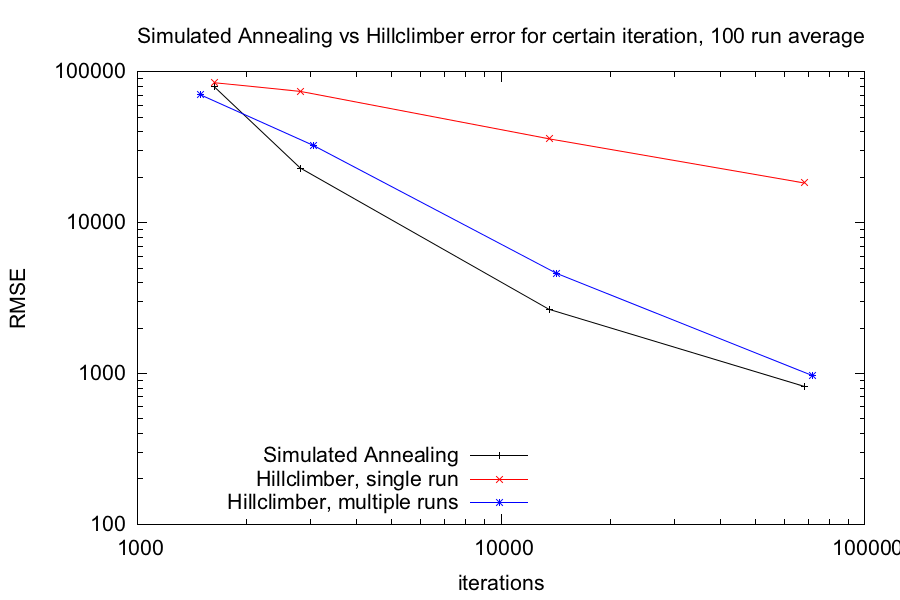
\includegraphics[width=2.5in]{iterations_vs_error_sa_hc}
\caption{Error for Simulated Annealing and Hill-climbing.}
\label{fig:error_sa_hc}
\end{figure}
\section{Conclusions}
\bibliographystyle{IEEEtran}
\bibliography{final_report}
\end{document}

